
	\Juan{Hablar de qué sirven los diodos y el cap.. si no recuerdo más es para un filtro y los diodos son por los picos altos que puede tener al ser un cap muy grande}
	\graficarEPS{0.6}{red_realim}{Red de realimentación propuesta.}{fig:red_realim}
	Se propone utilizar una realimentación negativa serie paralelo compuesto por las resistencias $R_{27}$ y $R_{15}$. Así se estabiliza el circuito en continua y también mejorar las características de amplificador de tensión (impedancia de entrada alta e impedancia de salida baja). Para limitar la corriente de base entrante al terminal inversor, el valor de $R_{27}$ debe ser del orden de las decenas de \si{\kilo\ohm}. Proponiendo los valores $R_{27}=\SI{22}{\kilo\ohm}$ y $R_{15}=\SI{1.1}{\kilo\ohm}$ se obtiene:

\begin{equation}
	\centering
	f = \frac{R_{15}}{R_{15} + R_{27}} = \frac{\SI{1.1}{\kilo\ohm}}{\SI{1.1}{\kilo\ohm} + \SI{22}{\kilo\ohm}} \approx \num{0.048}
\end{equation}

\begin{equation}
	\centering
	af = 0,048 \cdot 31200 = 1485 \implies af >> 1 \implies A \approx \frac{1}{f} = 21
\end{equation}

\subsection{Impedancia de salida}
	Con los valores obtenidos de la realimentación se calcula la impedancia de salida.

\begin{figure}[H]
	 \centering
	 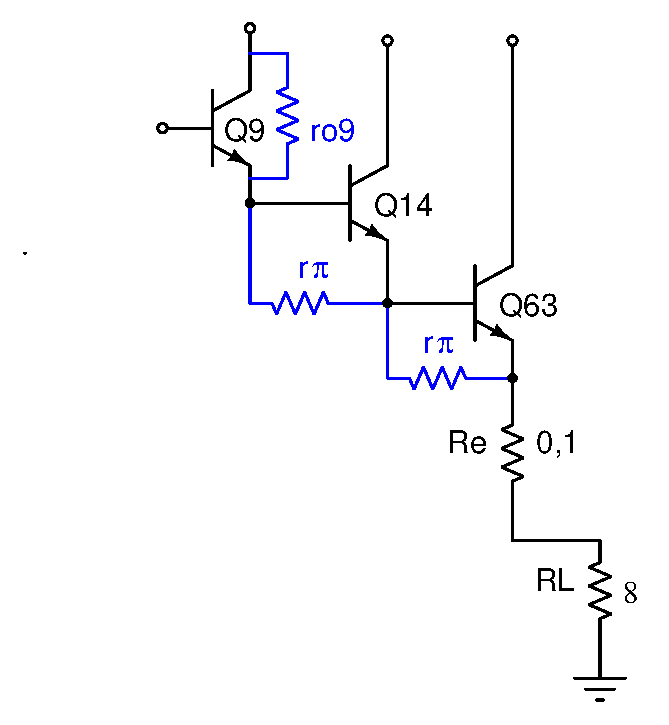
\includegraphics[scale=0.5]{ro.eps}
	 \caption{Diagrama para hallar la resistencia de salida del circuito sin realimentación.}
\end{figure}

\begin{itemize}
	\item Resistencia de salida sin realimentador: en esta situación se supone que, a los efectos de este cálculo, las resistencias de salida de los colectores comunes son iguales.
Entonces se calcula la resistencia de salida del circuito sin realimentar como
	\begin{equation}
		\centering
		R_o = \frac{1}{2} \cdot R_E + \frac{ r_{\pi}^{*} + r_{o,Q9} }{\beta^{*} } = \frac{1}{2} \left ( \SI{0.1}{\ohm} + \frac{\SI{32}{\kilo\ohm}}{75 \cdot 60} \right) = \SI{3.6}{\ohm}
	\end{equation}
	siendo
	\begin{equation}
		\centering
		r_{\pi}^{*} = 2 \cdot r_{\pi_{Q_{14}}} = 2 \cdot 60 \cdot \frac{25mV}{ \SI{110}{\milli\ampere}} = \SI{14}{\ohm} 
	\end{equation}
		
	%\begin{equation}
	%	\centering
	%	r_{o,Q9} = \frac{160V}{5mA} = \SI{32}{\kilo\ohm}
	%\end{equation}
		
	\item Resistencia de salida con realimentador
	\begin{equation}
		\centering
		R_{o,CR} = \frac{R_{o,SR}}{1+ af} = \frac{ \SI{3.6}{\ohm} }{1+1485} = \boxed{\SI{2.4}{\milli\ohm}} 
	\end{equation}
\end{itemize}


\subsection{Factor de amortiguamiento}

	En un sistema de audio, el factor de amortiguamiento es la relación entre la impedancia del altoparlante y la impedancia de salida del amplificador. Describe la capacidad del amplificador de controlar movimiento del altoparlante cuando se deja de excitarlo, en especial cercano a su frecuencia de resonancia. Este valor es de importancia en el contexto de las bajas frecuencias, o subwoofers, dado que la inercia de los diafragmas suele ser grande y el control de la suspensión débil, para permitir grandes excursiones.

\begin{equation}
	\centering
	f_a= \frac{Z_L}{Z_o} = \frac{ \SI{8}{\ohm}}{ \SI{2.4}{\milli\ohm}}= \boxed{\num{3333}}
	\label{ec:fa}
\end{equation}



\subsection{Resistencia de entrada}
	
	Con $R_{27}=\SI{22}{\kilo\ohm}$ el juego de resistores $R_{17}$ y $R_{18}$ deben sumar esa misma resistencia para compensar la tensión de corrimiento. Sin embargo, en un amplificador de audio se requiere que la impedancia de entrada sea alta. Se propone un \emph{bootstrap} entre los pines inversor y no-inversor para aumentar dicha resistencia, colocando $C_8$. Para evitar oscilasiones al unir dichas entradas se conecta $R_{20}$.
	

\begin{itemize}
	
	\HgraficarEPS{0.5}{ri}{Diagrama en bloque para hallar la resistencia de entrada.}{fig.esq_ri}
		
\item \textbf{Resistencia de entrada sin realimentación}
	
	\begin{equation}
		\centering
		R_{i,SR} = \SI{100}{\ohm} + R_{F1}//R_{F2} = \SI{100}{\ohm} + \SI{22}{\kilo\ohm}//\SI{1.1}{\kilo\ohm}
	\end{equation}
	
\item \textbf{Resistencia de entrada con realimentación}
	\HgraficarEPS{0.5}{ri_realim}{Diagrama en bloque para hallar la resistencia de entrada.}{fig.esq_ri_f}
	\begin{equation}
		\centering
		R_{i,CR} = (1+ af) \cdot R_{i,SR} = (1 + 1485) \cdot \SI{1.1}{\kilo\ohm} = \SI{1.6}{\mega\ohm}
	\end{equation}
	
\end{itemize}

Finalmente la resistencia que ve el generador es

$$ \SI{100}{\kilo\ohm}//\SI{1.6}{\mega\ohm} = \boxed{\SI{94}{\kilo\ohm}} $$



